% !TeX document-id = {d7bfea81-c3f6-4000-b3a4-ebfa033e41d4}
% !TeX root = ./main.tex
% !TEX program = xelatex
% !BIB program = biber
% !TEX encoding = UTF-8 Unicode
% !TEX options = --shell-escape -synctex=1 -interaction=nonstopmode -file-line-error "%DOC%"
\documentclass{kuee_en}

% if your prefer Times New Roman in Windows, pleas uncomment the below two lines.
% \usepackage{fontspec}
% \setmainfont{Times New Roman}
% and comment these two line
\usepackage[T1]{fontenc}
\usepackage{mathptmx}

\usepackage{setspace}
%\singlespacing % 43 lines per page
\setstretch{1.2} % 36 lines per page
%\onehalfspacing % 33 line per page


% using modern biblatex
\bibliography{sample}

\title{An English \LaTeX{} Template for KUEE}
\etitle{An English \LaTeX{} Template for KUEE}
\eauthor{Denki Jiro} 
\author{{電気 次郎}} % if no kanji name, remove  env.
\supervisor{{電気 太郎 教授}}
\school{{京都大学大学院工学研究科}}
\depart{{電子工学専攻}}
\date{{令和2年2月1日}}

\begin{document}
\maketitle

\begin{abstract}
    \lipsum[1]
\end{abstract}

\tableofcontents

\chapter{Usage}

This template is designed for the english writer for master thesis in KUEE. All the formats are referred to the Japanese guide of master thesis.\footnote{修士論文作成規定および手引, 2019年12月13日改定}
In the case of PhD students, it is free to use any \LaTeX ~template as I know in KUEE. For undergraduate students, I think only Japanese is acceptable. If necessary, it easy to change the title in \verb|kuee_en.cls| file.
\footnote{Hint, line 37}

The default compiler of this template is \verb|xelateX| as magic commands are defined in the file head. This is due to the use of \verb|xeCJK| and \verb|fontspec| packages. If you want old-fashion \verb|pdflatex| or \verb|latex|, please note the package compatibility.

\section{Line spacing}
The required lines in Japanese version is about 32. While default \verb|a4paper| using single spacing in \LaTeX means more than 40 lines per page. Despite the language difference, 1.2 line spacing is recommended. You can also change this value in the macro of package \verb|setspace|. You can check it with contents in chapter 2.



\section{CJK Languages}

\verb|xeCJK| is used in this paper to generate the cover page. Default font is Meicho font.
This is an example of quotation.
\begin{quote}
電気電子工学は現代のあらゆる産業や社会生活の基盤として欠くことのできない科学技術となっています
\end{quote}

\section{Formula for scientists}
A modern package \verb|physics| is added into the style file. It is much easier to give some fractions and notation in physics.
 
Multiple-line aligned example, Maxwell Equations
\begin{align}
    \div{\vb{D}} &= 0 \\
    \div{\vb{B}} &= 0 \\
    \curl{\vb{E}} &= -\pdv{\vb{B}}{t} \\
    \curl{\vb{H}} &= \pdv{\vb{D}}{t}
\end{align}

Schr\"{o}edinger Equation
\begin{equation}
	i\hbar \pdv{\ket{\varphi}}{t} = \mathcal{H} \ket{\varphi}
\end{equation}

Chemical equation example
\begin{equation*}
    2\ce{H2}+\ce{O2} = 2\ce{H2O}
\end{equation*}

\section{Reference and Citation}
Cite this paper
\cite{Yang2007}

\section{Figure and Graph}
A tikz figure shown in Fig. \ref{fig:tikz} and automatically floated to the file end.

\begin{figure}
    \centering
    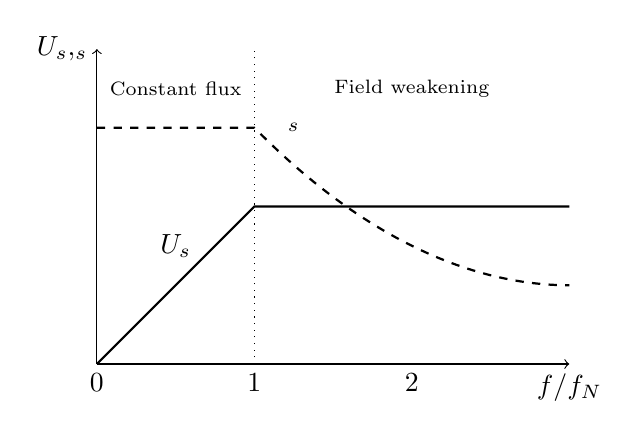
\begin{tikzpicture}
    % horizontal axis
    \draw[->] (0,0) -- (6,0) node[anchor=north] {$f/f_N$};
    % labels
    \draw	(0,0) node[anchor=north] {0}
    		(2,0) node[anchor=north] {1}
    		(4,0) node[anchor=north] {2};
    % ranges
    \draw	(1,3.5) node{{\scriptsize Constant flux}}
    		(4,3.5) node{{\scriptsize Field weakening}};
    % vertical axis
    \draw[->] (0,0) -- (0,4) node[anchor=east] {$U_s,\varPsi_s$};
    % nominal speed
    \draw[dotted] (2,0) -- (2,4);
    % Us
    \draw[thick] (0,0) -- (2,2) -- (6,2);
    \draw (1,1.5) node {$U_s$}; %label
    % Psis
    \draw[thick,dashed] (0,3) -- (2,3) parabola[bend at end] (6,1);
    \draw (2.5,3) node {$\varPsi_s$}; %label
    \end{tikzpicture}
  \caption{A tikz figure example}
  \label{fig:tikz}
\end{figure}


\section{Layout and Parameters}
Default parameters used in this template is shown in Tab.\ref{tab:text}, Tab.\ref{tab:fig}.

\begin{table}
  \caption{Default layout}\label{tab:text}
  \begin{center}
    \begin{tabular}{|l|r|}
      \hline
      \verb+\textwidth+ & 424pt \\ \hline
      \verb+\textheight+ & 604pt \\ \hline
      \verb+\oddsidemargin+ & 0.5cm \\ \hline
      \verb+\evensidemargin+ & 0.5cm \\ \hline
      \verb+\topmargin+ & 0pt \\ \hline
      \verb+\headheight+ &12pt \\ \hline
      \verb+\headsep+ & 25pt \\ \hline
      \verb+\footskip+ & 30pt \\ \hline
    \end{tabular}
  \end{center}
\end{table}

\begin{table}
  \caption{Default parameters for graphs}\label{tab:fig}
  \begin{center}
    \begin{tabular}{|l|r|}
      \hline
      \verb+\textwidth+ & 424pt + 1cm \\ \hline
      \verb+\textheight+ & 604pt + 67pt \\ \hline
      \verb+\oddsidemargin+ & 0pt \\ \hline
      \verb+\evensidemargin+ & 0pt \\ \hline
      \verb+\topmargin+ & 0pt \\ \hline
      \verb+\headheight+ & 0pt \\ \hline
      \verb+\headsep+ & 0pt \\ \hline
      \verb+\footskip+ & 0pt \\ \hline
    \end{tabular}
  \end{center}
\end{table}


\chapter{Lorem Ipsum}
\lipsum[1-10]


\begin{acknowledgements}
\lipsum[2]
\end{acknowledgements}

\printbibliography[title=References,heading=bibintoc]

\clearpage % ensure all floats are processed
\processdelayedfloats
\clearpage

\begin{appendices}
\chapter{Versions}
\begin{description}
  \item[2019] 1st version by Zhenghao Yin, Takeuchi lab.
\end{description}
\end{appendices}


\end{document}

